\documentclass[12pt, a4paper]{article}

% Pacchetti base consigliati
\usepackage[utf8]{inputenc}
\usepackage[italian]{babel}
\usepackage{graphicx} % Essenziale per inserire le immagini
\usepackage{geometry}
\usepackage{svg}
\geometry{a4paper, margin=2.5cm}
\usepackage{hyperref}

\title{\textbf{Assignment 02 - Smart Drone Hangar}}
\author{Cattolico Giuseppe, Muller Arthur}
\date{\today}

\begin{document}

\maketitle

\section{Introduzione e Obiettivo}
Il progetto "Smart Drone Hangar" ha l'obiettivo di realizzare un sistema embedded per la gestione automatizzata del decollo e dell'atterraggio di un drone. Il sistema è suddiviso in due macro-componenti interconnessi tramite linea seriale: un'unità di controllo locale basata su Arduino (Drone Hangar), incaricata di gestire i sensori e gli attuatori fisici, e un'unità remota su PC (Drone Remote Unit - DRU) dotata di interfaccia grafica (GUI) per l'invio dei comandi e il monitoraggio dello stato. L'intero firmware Arduino è stato progettato seguendo un'architettura basata su task concorrenti e Macchine a Stati Finiti (FSM) sincrone, garantendo reattività e una corretta temporizzazione delle operazioni.

\section{Architettura Hardware}

\subsection{Schema Elettrico e Breadboard}

\begin{figure}[h!]
    \centering
    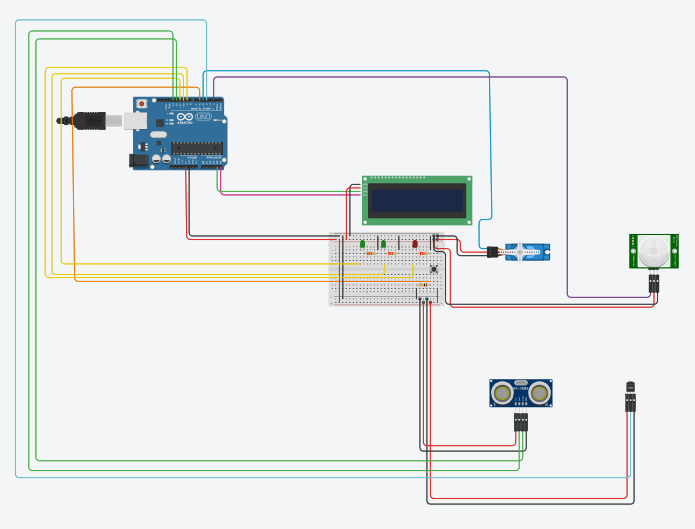
\includegraphics[width=0.8\textwidth]{svg/assignment-2-ThinkerCad.png}
    \caption{Rappresentazione della breadboard e schema circuitale.}
    \label{fig:schema_hw}
\end{figure}

\subsection{Descrizione dei Componenti e Pin mapping}
Il sottosistema locale si avvale dei seguenti componenti fisici per mappare l'ambiente e interagire con l'operatore. Di seguito è riportato il dettaglio dei collegamenti hardware al microcontrollore:

\begin{itemize}
    \item \textbf{PIR Sensor (DPD) - \texttt{Pin 2}:} Rileva la presenza fisica del drone in prossimità della sommità dell'hangar durante le fasi di atterraggio.
    \item \textbf{Sensore Sonar (DDD) - \texttt{Trig: Pin 13, Echo: Pin 12}:} Misura costantemente la distanza del drone quando si trova all'interno o in prossimità della base, permettendo di validare l'effettivo completamento del decollo o dell'atterraggio. 
    \item \textbf{Servo Motore (HD) - \texttt{Pin 5}:} Attuatore che controlla l'apertura e la chiusura della porta dell'hangar.
    \item \textbf{Display LCD I2C (16x2) - \texttt{Indirizzo 0x27}:} Fornisce un feedback visivo immediato all'operatore locale sullo stato del sistema (es. \textit{DRONE INSIDE}, \textit{TAKE OFF}, \textit{ALARM}).
    \item \textbf{Sensore di Temperatura (TEMP) - \texttt{Pin 4}:} Monitora le condizioni termiche interne per prevenire surriscaldamenti durante le fasi operative.
    \item \textbf{LED di Segnalazione - \texttt{L1: Pin 9, L2: Pin 10, L3: Pin 11}:} L1 (verde) indica l'operatività del sistema, L2 (verde) lampeggia con periodo di 0.5s durante le manovre di decollo/atterraggio, e L3 (rosso) segnala uno stato di allarme critico.
    \item \textbf{Pulsante Tactile (RESET) - \texttt{Pin 6}:} Permette all'operatore di ripristinare il sistema in seguito alla risoluzione di un'anomalia termica.
\end{itemize}

\section{Architettura Software}

\subsection{Struttura del Sistema}
Il firmware è strutturato in task cooperativi eseguiti da uno scheduler personalizzato. Questa scelta architetturale permette di gestire in modo non bloccante la lettura dei sensori (Sonar, PIR, Temperatura), il controllo del servomotore, l'aggiornamento dell'interfaccia LCD e la comunicazione bidirezionale tramite porta seriale con l'applicazione PC. Il comportamento logico del sistema è governato da macchine a stati finiti che valutano le transizioni in base agli input dei sensori, ai comandi ricevuti dal DRU e a specifici timeout temporali (T1, T2, T3, T4).
\newpage
\subsection{Diagrammi delle Macchine a Stati (FSM)}
\begin{figure}[h!]
    \centering
    
\includegraphics[width=0.8\linewidth]{svg/state-bg.png}
    \caption{Diagramma della Macchina a Stati Finiti del sistema.}
    \label{fig:fsm_diagram}
\end{figure}

\newpage
\subsection{I 4 Task Concorrenti e il loro Funzionamento}
Il sistema è stato suddiviso in quattro task indipendenti, ognuno con una precisa responsabilità operativa (Separation of Concerns), descritti di seguito:

\begin{itemize}
    \item \textbf{MainHangarTask (Logica di Movimento):} Gestisce il comportamento primario del hangar. Reagisce ai comandi (\texttt{takeOffCommand}, \texttt{landingCommand}) a condizione che non vi siano allarmi attivi. Attende le conferme spaziali e temporali dai sensori (Sonar e PIR) per completare le transizioni di stato. Si occupa inoltre di pilotare il servomotore della porta e aggiornare il display LCD.
    \item \textbf{AlarmTask (Monitoraggio Sicurezza):} Valuta costantemente la temperatura in modo slegato dalle operazioni di volo. In caso di innalzamento termico, porta il sistema in \textit{Pre-alarm} (inibendo nuove manovre) o in \textit{Alarm} (bloccando qualsiasi azione, chiudendo la porta e accendendo il LED rosso L3 fino alla pressione del tasto di reset).
    \item \textbf{BlinkingLedTask (Feedback Visivo):} Fa lampeggiare il LED verde L2 durante le fasi transitorie. Controlla continuamente se il sistema è in fase di decollo o atterraggio e, in caso affermativo, alterna lo stato del LED ogni 250ms, generando un periodo complessivo di 500ms.
    \item \textbf{SerialTask (I/O e Comunicazione):} Gestisce la comunicazione con l'unità remota (DRU). Ascolta i comandi in arrivo (es. \texttt{TAKEOFF}, \texttt{LAND}) e invia periodicamente (ogni 500ms) una stringa di riepilogo con lo stato aggiornato dell'hangar.
\end{itemize}

\subsection{Vantaggi dell'Architettura a Task}
L'adozione di una soluzione basata su 4 task cooperativi garantisce tre vantaggi fondamentali rispetto a un tradizionale approccio monolitico:
\begin{enumerate}
    \item \textbf{Esecuzione non bloccante:} Evitando l'uso di funzioni bloccanti come \texttt{delay()}, lo scheduler può eseguire operazioni periodiche (come il lampeggio del LED) senza impedire al microcontrollore di continuare a leggere sensori o ascoltare la seriale.
    \item \textbf{Affidabilità della Sicurezza:} L'\texttt{AlarmTask} viene eseguito in parallelo. Ciò assicura che il controllo termico non venga mai interrotto o ritardato dalle tempistiche meccaniche della porta o da eventuali latenze di lettura degli stati da parte della DRU.
    \item \textbf{Modularità:} La netta separazione delle logiche rende il firmware facilmente manutenibile ed espandibile.
\end{enumerate}

\subsection{Gestione dello Stato Condiviso: Il Context}
Per far comunicare i task senza accoppiarli rigidamente, è stato implementato il pattern architetturale \textit{Shared State Object} tramite la classe \texttt{Context}. I task non comunicano mai direttamente tra loro. Il \texttt{Context} funge da "bacheca condivisa":
\begin{itemize}
    \item \textbf{Scrittura:} Il \texttt{SerialTask} riceve un comando e invoca, ad esempio, \texttt{setTakeOffCommand()}, demandando l'esecuzione effettiva.
    \item \textbf{Lettura:} Il \texttt{MainHangarTask} interroga ciclicamente il \texttt{Context} (\texttt{isTakeOffCommanded()}) per avviare le proprie routine, mentre il \texttt{BlinkingLedTask} legge flag come \texttt{isTakingOff()} per avviare il lampeggio.
\end{itemize}
Questo approccio nasconde l'implementazione delle singole variabili e mantiene il sistema coerente e disaccoppiato.

\subsection{Comunicazione Seriale: DRU e Hangar}
Il sistema di comunicazione tra la GUI su PC (DRU) e l'hardware (Hangar) si basa su un'architettura seriale bidirezionale e asincrona a 115200 baud. Il protocollo è progettato per essere rigorosamente non bloccante in entrambi gli ambienti, affidandosi al carattere terminatore di a capo (\texttt{\textbackslash n}) per identificare la fine di ogni pacchetto dati.

\textbf{Lato PC (Drone Remote Unit in Java):}
La DRU sfrutta un'architettura multi-thread per separare la ricezione dei dati dall'interfaccia grafica:
\begin{itemize}
    \item \textbf{Invio Comandi:} Il \texttt{DashboardController} elabora gli input dell'utente e trasmette le stringhe di comando (es. \texttt{TAKEOFF}) tramite la classe \texttt{SerialCommChannel}, accodando sempre il terminatore \texttt{\textbackslash n}.
    \item \textbf{Ricezione Asincrona:} I byte in ingresso scatenano un evento hardware (\texttt{serialEvent}). I caratteri vengono bufferizzati e, non appena viene rilevato un \texttt{\textbackslash n}, la stringa completa viene estratta e inserita in una \texttt{BlockingQueue} thread-safe.
    \item \textbf{Elaborazione e GUI:} Un thread parallelo, il \texttt{MonitoringAgent}, preleva continuamente i messaggi dalla coda. Se rileva una stringa di telemetria (formattata con campi separati da \texttt{|}), ne effettua il parsing e aggiorna i pannelli della dashboard e il file di log senza mai bloccare il thread grafico principale (\textit{Event Dispatch Thread}).
\end{itemize}

\textbf{Lato Arduino (SerialTask e MsgService):}
Il microcontrollore gestisce i messaggi seriali senza interrompere l'esecuzione dei task critici (come l'\texttt{AlarmTask}):
\begin{itemize}
    \item \textbf{Ascolto in Background:} La funzione nativa \texttt{serialEvent()} accumula i caratteri in arrivo in un buffer testuale in modo del tutto silente. Solo alla ricezione del terminatore \texttt{\textbackslash n}, la stringa viene impacchettata in un oggetto \texttt{Msg} e viene alzato il flag \texttt{msgAvailable}.
    \item \textbf{Gestione nel Task:} Il \texttt{SerialTask}, durante il suo \textit{tick} operativo, chiama il metodo \texttt{isMsgAvailable()}. Se il flag è attivo, ritira il comando e lo inoltra al \texttt{Context} (es. impostando il flag di decollo).
    \item \textbf{Invio Telemetria:} Ogni 500ms, il task assembla la stringa di stato (es. \texttt{STATE:...|HANGAR:...|DIST:...}) e la invia con \texttt{MsgService.sendMsg()}, la quale esegue internamente una \texttt{Serial.println()} aggiungendo automaticamente il \texttt{\textbackslash n} atteso dal PC.
\end{itemize}

\section{Note Operative}

\subsection{Note Operative e Parametrizzazione}
Il prototipo è stato sviluppato tenendo in forte considerazione la flessibilità in fase di test e calibrazione. Tutti i parametri fisici e temporali richiesti dalle specifiche (\textit{D1, D2, T1, T2, T3, T4, Temp1, Temp2}) sono stati implementati come costanti (\texttt{\#define}) o variabili di configurazione facilmente modificabili.


\section{Difficoltà Riscontrate e Conclusioni}

\subsection{Difficoltà Riscontrate}
Durante la fase di sviluppo e implementazione del prototipo, abbiamo affrontato e risolto diverse sfide tecniche, sia hardware che software:

\begin{itemize}
    \item \textbf{Lettura dei sensori e librerie esterne:} Abbiamo optato per l'utilizzo di un sensore di temperatura DHT11. Tuttavia, l'integrazione di questo componente e delle relative librerie di terze parti ha causato difficoltà nella lettura dei dati, introducendo latenze e conflitti con la natura della nostra architettura a task.
    \item \textbf{Gestione dello stato condiviso:} Nelle prime iterazioni del codice, la classe \texttt{Context} non era strutturata in modo del tutto completo. Questo ha generato alcune difficoltà nel corretto aggiornamento e nella sincronizzazione delle variabili di stato, portando a comportamenti imprevisti. La revisione e il completamento del pattern \textit{Shared State} hanno poi risolto definitivamente questi conflitti tra task.
    \item \textbf{Letture anomale del Sonar (Overflow):} Abbiamo riscontrato un'anomalia fisica legata al sensore a ultrasuoni. Quando la porta dell'hangar era aperta e non vi erano ostacoli vicini, il Sonar misurava una distanza fuori scala, restituendo un valore negativo che corrompeva la logica di controllo (simulando falsamente l'avvenuto atterraggio/decollo). Come visibile nel video allegato, abbiamo risolto il problema in modo pratico posizionando un oggetto dietro la porta aperta, garantendo così una lettura di "background" fissa e sicura per il sensore.
    \item \textbf{Comunicazione Seriale PC-Arduino:} L'implementazione dell'interfaccia di comunicazione tra l'applicazione Java (GUI remota) e la porta seriale di Arduino ha richiesto particolare attenzione. Si sono verificati problemi iniziali di sincronizzazione e perdita di pacchetti tra i due ambienti.
\end{itemize}

\subsection{Conclusioni}
Lo sviluppo dello \textit{Smart Drone Hangar} ha confermato la netta superiorità di un'architettura software basata su task concorrenti e Macchine a Stati Finiti (FSM) rispetto a un approccio procedurale monolitico. 

Nonostante le difficoltà iniziali legate all'integrazione dei sensori e alla comunicazione seriale, la separazione delle responsabilità (\textit{Separation of Concerns}) tra logica di movimentazione, sicurezza termica e I/O ha permesso di isolare e risolvere i bug in modo mirato.

In conclusione, il sistema finale risulta reattivo e deterministico: i task critici, come l'\texttt{AlarmTask}, intervengono tempestivamente senza mai essere ritardati o interrotti dalle operazioni meccaniche del servomotore o da eventuali latenze della GUI remota.

\end{document}